\chapter{IMUs}\label{cha2}

For estimating the kite's state measurements from different sensors are needed. An inertial measurement unit (IMU) contains several sensors that measure physical quantities like acceleration, rate of turn, a magnetic field or ambient air pressure. There are many different such IMU's available, which may be distinguished by which sensors are embedded, at what rate they provide the data, what is their range and sensitivity and how much signal processing is done internally.

The Swiss Kite Power Project has the following options of IMUs to choose:

\begin{description}
\item[MTi-G]
The MTi-G development kit is a commercial product from the Dutch company Xsens. The unit has an accelerometer, gyroscope, magnetometer, pressure sensor and GPS with antenna included. It exist two output data formats. It can be chosen wether the output is raw data or calibrated data. The calibrated data from the sensors without GPS gives the data in common units and uses a calibration to compensate offsets. In addition, the GPS and IMU data can be processed with an Extended Kalman Filter resulting in a filtered output of position and attitude.

\item[PX4]
The PX4 is a open-source/open-hardware IMU used and developed by the PIXHAWK Project of the Computer Vision and Geometry Lab of ETH Zurich. The unit contains a temperature and pressure sensor, an accelerometer, a gyroscope and a magnetometer. The IMU additionally provides a counter for each sensor to ensure an easy handling of the different output frequencies of the included sensors. The output of the sensors is raw data. In the estimation algorithm (see chapter \ref{cha3}) only the embedded accelerometer a BMA180 from Bosch (see the data sheet in appendix \ref{ds_acc}), the gyroscope a L3GD20 from STMicroelectronics (see the data sheet in appendix \ref {ds_gyro}) and the magnetometer a HMC5883L from Honeywell(see the data sheet in appendix \ref{ds_mag}) are used.

\item[x-IMU]
The x-IMU is a product of the company x-io Technologies. It also has a temperature sensor, an accelerometer, a gyroscope and a magnetometer. The configuration of the x-IMU was done by the FHNW. It provides only raw data. The data sheets of the sensors can be found in the appendix \ref{ds_ximu}.
\end{description}


\section{Centrifuge Test}
There are several performance requirements on an IMU installed on a kite. One of them is the dependency on g-loads because on a kite several g loads can appear. Therefore a centrifuge test was carried out in corporation with the Fachhochschule Nordwestschweiz (FHNW)
\subsection{Set-up}
The setting of the centrifuge is described in (…..Figure.....). It was provided by the FHNW. An arm is rotated by a motor. The IMUs are mounted in a box at the end of the arm. The sensors are put next to each other to have similar measurements in all sensors. A Pictture of the Box can be seen in Figure (….Figure....). Obviously, the motion of the box is describing a circle with a radius (the distance between the rotation axis and the  center of the box) of $0.75 m$. The motor is able to rotate the arm with a velocity of about $10 m/s$. Which corresponds to a maximum acceleration of about $ a=\omega*r^2=8 g$. 

Even though a sensor on the centrifuge was measuring the rate of turn, there was no software for the data collection implemented. Therefore we have no ground truth to compare the sensor data with. 
During the test, the motor was driven in order to have 5 steps between $1.62 g$ and $7.8 g$ $(ca. 1.6 g; 2.4 g 3.7 g; 5.4 g; 6.9 g; 7.8 g)$ of centripetal acceleration.

The PX4 and Xsens are connected together. Both, the PX4 and the Xsens measurements are written on the SD card of the PX4 Unit. The timestamps for the sensor readings are taken from the GPS clock for the Xsens as well as for the PX4 at the time when they are logged on the SD card. This results in easy and accurate synchronization between the two IMUs. To get the time synchronized with the third IMU, the x-IMU is synchronized to the computer's time. Additionally the 3 sensors are hit for having a clearly distinghuishable signal aiding in the estimation of how accurate the synchronization is.
\subsection{Result}
The raw data from the x-IMU is scaled by Raphael Mueller bringing it to the common units $m/s^2$ for the accelerometer, $deg/s$ for the gyroscope and $gauss$ for the magnetometer.

The PX4 was set by the group of the PixHawk Project. How the output of the sensors have to be scaled to bring them in the required units is shown in table \ref{ct_units_PX4}. The scale factor describes by how much the output has to be multiplied to get the data converted in the units described in 4th row.
\begin{table}[h]
\centering
\begin{tabular}{|p{2.5 cm}|c|c|c|p{3 cm}|}
 \hline
 Sensor & Sensitivity & Scale Factor & Unit & Comment \\
 \hline
 Accelerometer BMA180 & $2048 LSB/g$ & $output*9.81/2048$ & $m/s^2$ &     Sensitivity range: $+/- 4 g$ \\
 \hline
 Gyroscope L3GD20 & $17.5 mdps/digit$ & $output*17.5/1000$ & $deg/s$ &   \\
 \hline
 Magnetometer HMC5883L & $1370 LSB/g$ & $output/1370$ & gauss &   \\
\hline
\end {tabular}
\caption{This table shows how the raw data output of the PX4 has to be sclaed to get the right units.}
\label{ct_units_PX4}
\end{table}
The MTi-G has also raw output data but no clear explanation in the data sheet (…..) on how to get to the required units. Therefore, were the MTi-G data scaled to bring it more or less to the same order as the other two IMUs are.
In (...figure...) we can see the plot of the GPS data.
\begin{figure}[h]
\begin{center}
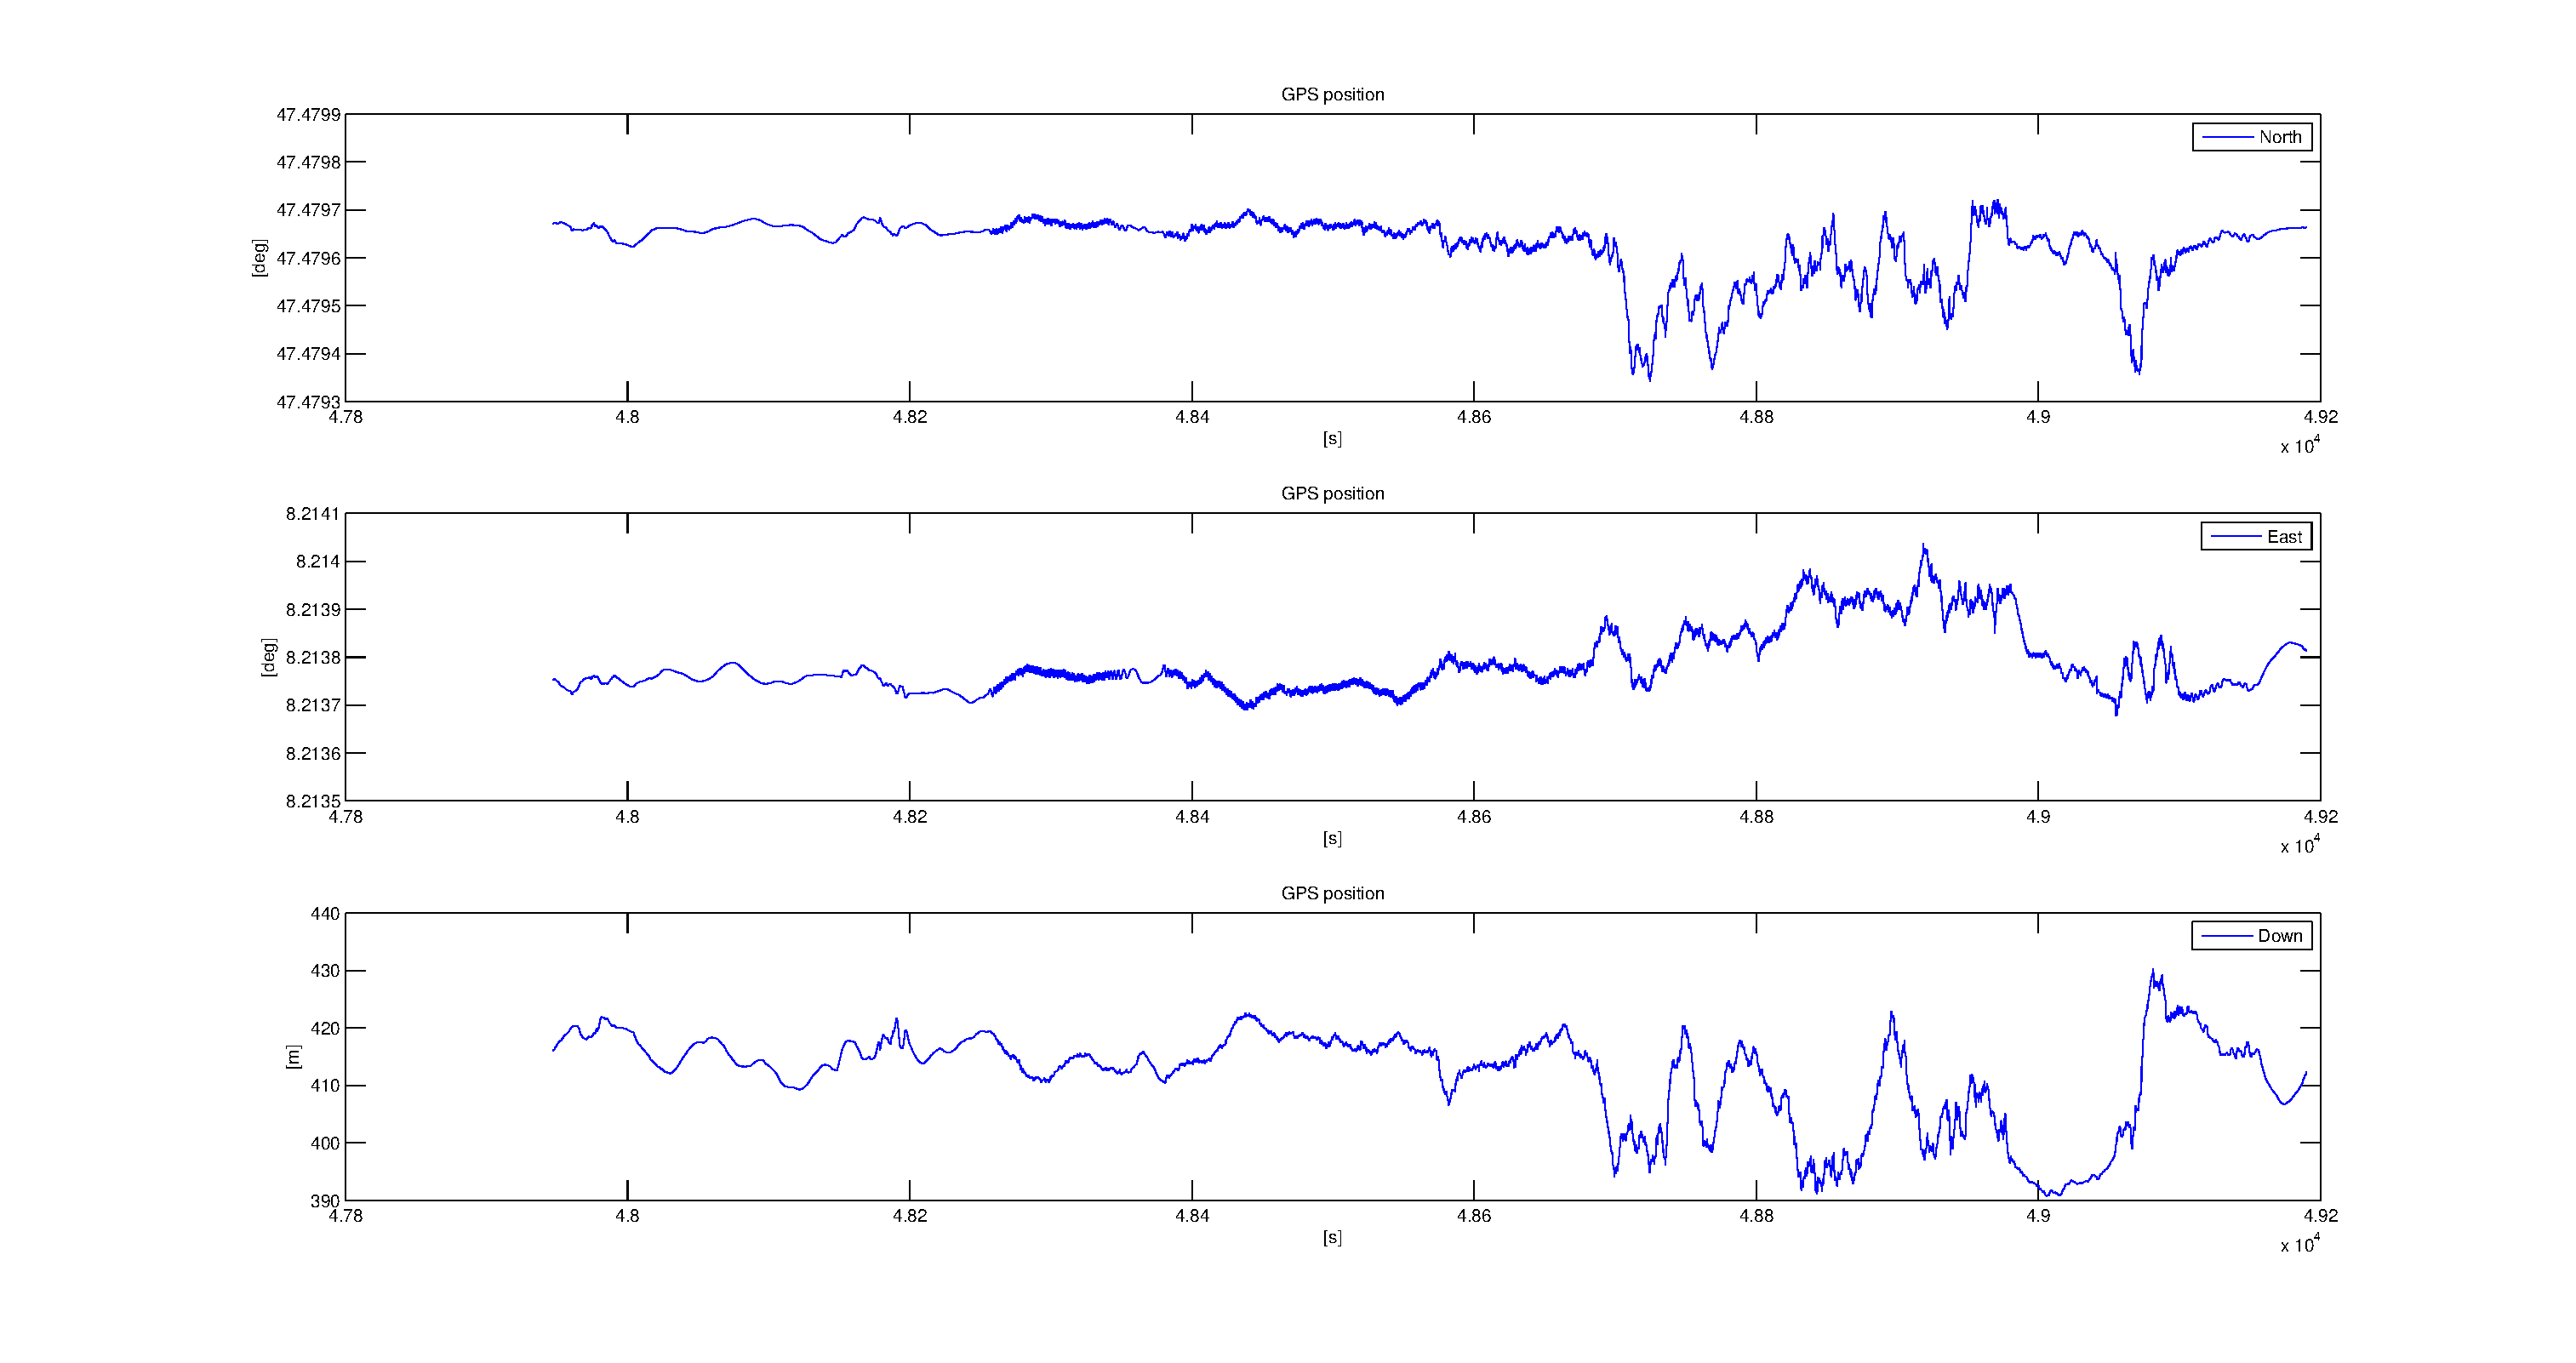
\includegraphics[width=1.2\textwidth]{pictures/ct_pos.eps}
\caption{GPS Position}
\label{ct_pos}
\end{center}
\end{figure}
Until 4.83e4 s is the centrifuge not in motion. The mean value of this period is the taken as the ground truth to calculate the the average error of the GPS signal. The mean value of the north component is $47.48 deg$ for the east component $8.2138 deg$ and for the down component $415.74 m$. The coordinates of Winidsch, where the test takes place is $47.4806 deg$, $8.2222 deg$ and $357 m$. By taking the average absolute difference between the GPS data and the mean value calculated before, an error of the GPS can be estimated: $1.08*10^{-5} deg$, $1.37*10^{-5}deg$ and $2.49 m$ for north, east, down respectively. After $4.83*10^{4} s$ the noise is increasing. At this time the centrifuge starts rotating. The calculated  errors in this period are: $1.68*10^{-5} deg$, $2.27*10^{-5} deg$ and $2.89 m$ for north east, down respectively. After $4.87*10^{4} s$ the noise look very high. This is when we have  a centripetal acceleration of more than  $6.7 g$. The estimated noise is: $1.04*10^{-4} deg$, $1.02*10^{-4} deg$ and $13.01 m$. Since in non of this periods a cosine of sine behavior of the north and east component can be seen all three components should be stable in the ideal case. The error values a summarized in table \ref{ct_pos_error}.
\begin{table}[h]
\centering
\begin{tabular}{|l|r|}
\hline
Period & Average error (north/east/down) \\
\hline
$4.80*10^{4} s - 4.83*10^{4} s$&$1.08*10^{-5} deg / 1.37*10^{-5} deg / 2.49 m$\\
\hline
$4.83*10^{4} s – 4.87*10^{4} s$&$1.68*10^{-5} deg / 2.27*10^{-5} deg / 2.89 m$\\
\hline
$4.87*10^{4} s – 4.91*10^{4} s$&$1.04*10^{-4} deg/ 1.02*10^{-4} deg / 13.01 m$\\
\hline
\end{tabular}
\caption{The average error of the postion in different time segments}
\label{ct_pos_error}
\end{table}
Due to the fact that the velocity is the derivative of the position of the GPS the amplitude of the error behaves  similar.
\begin{figure}[h]
\centering
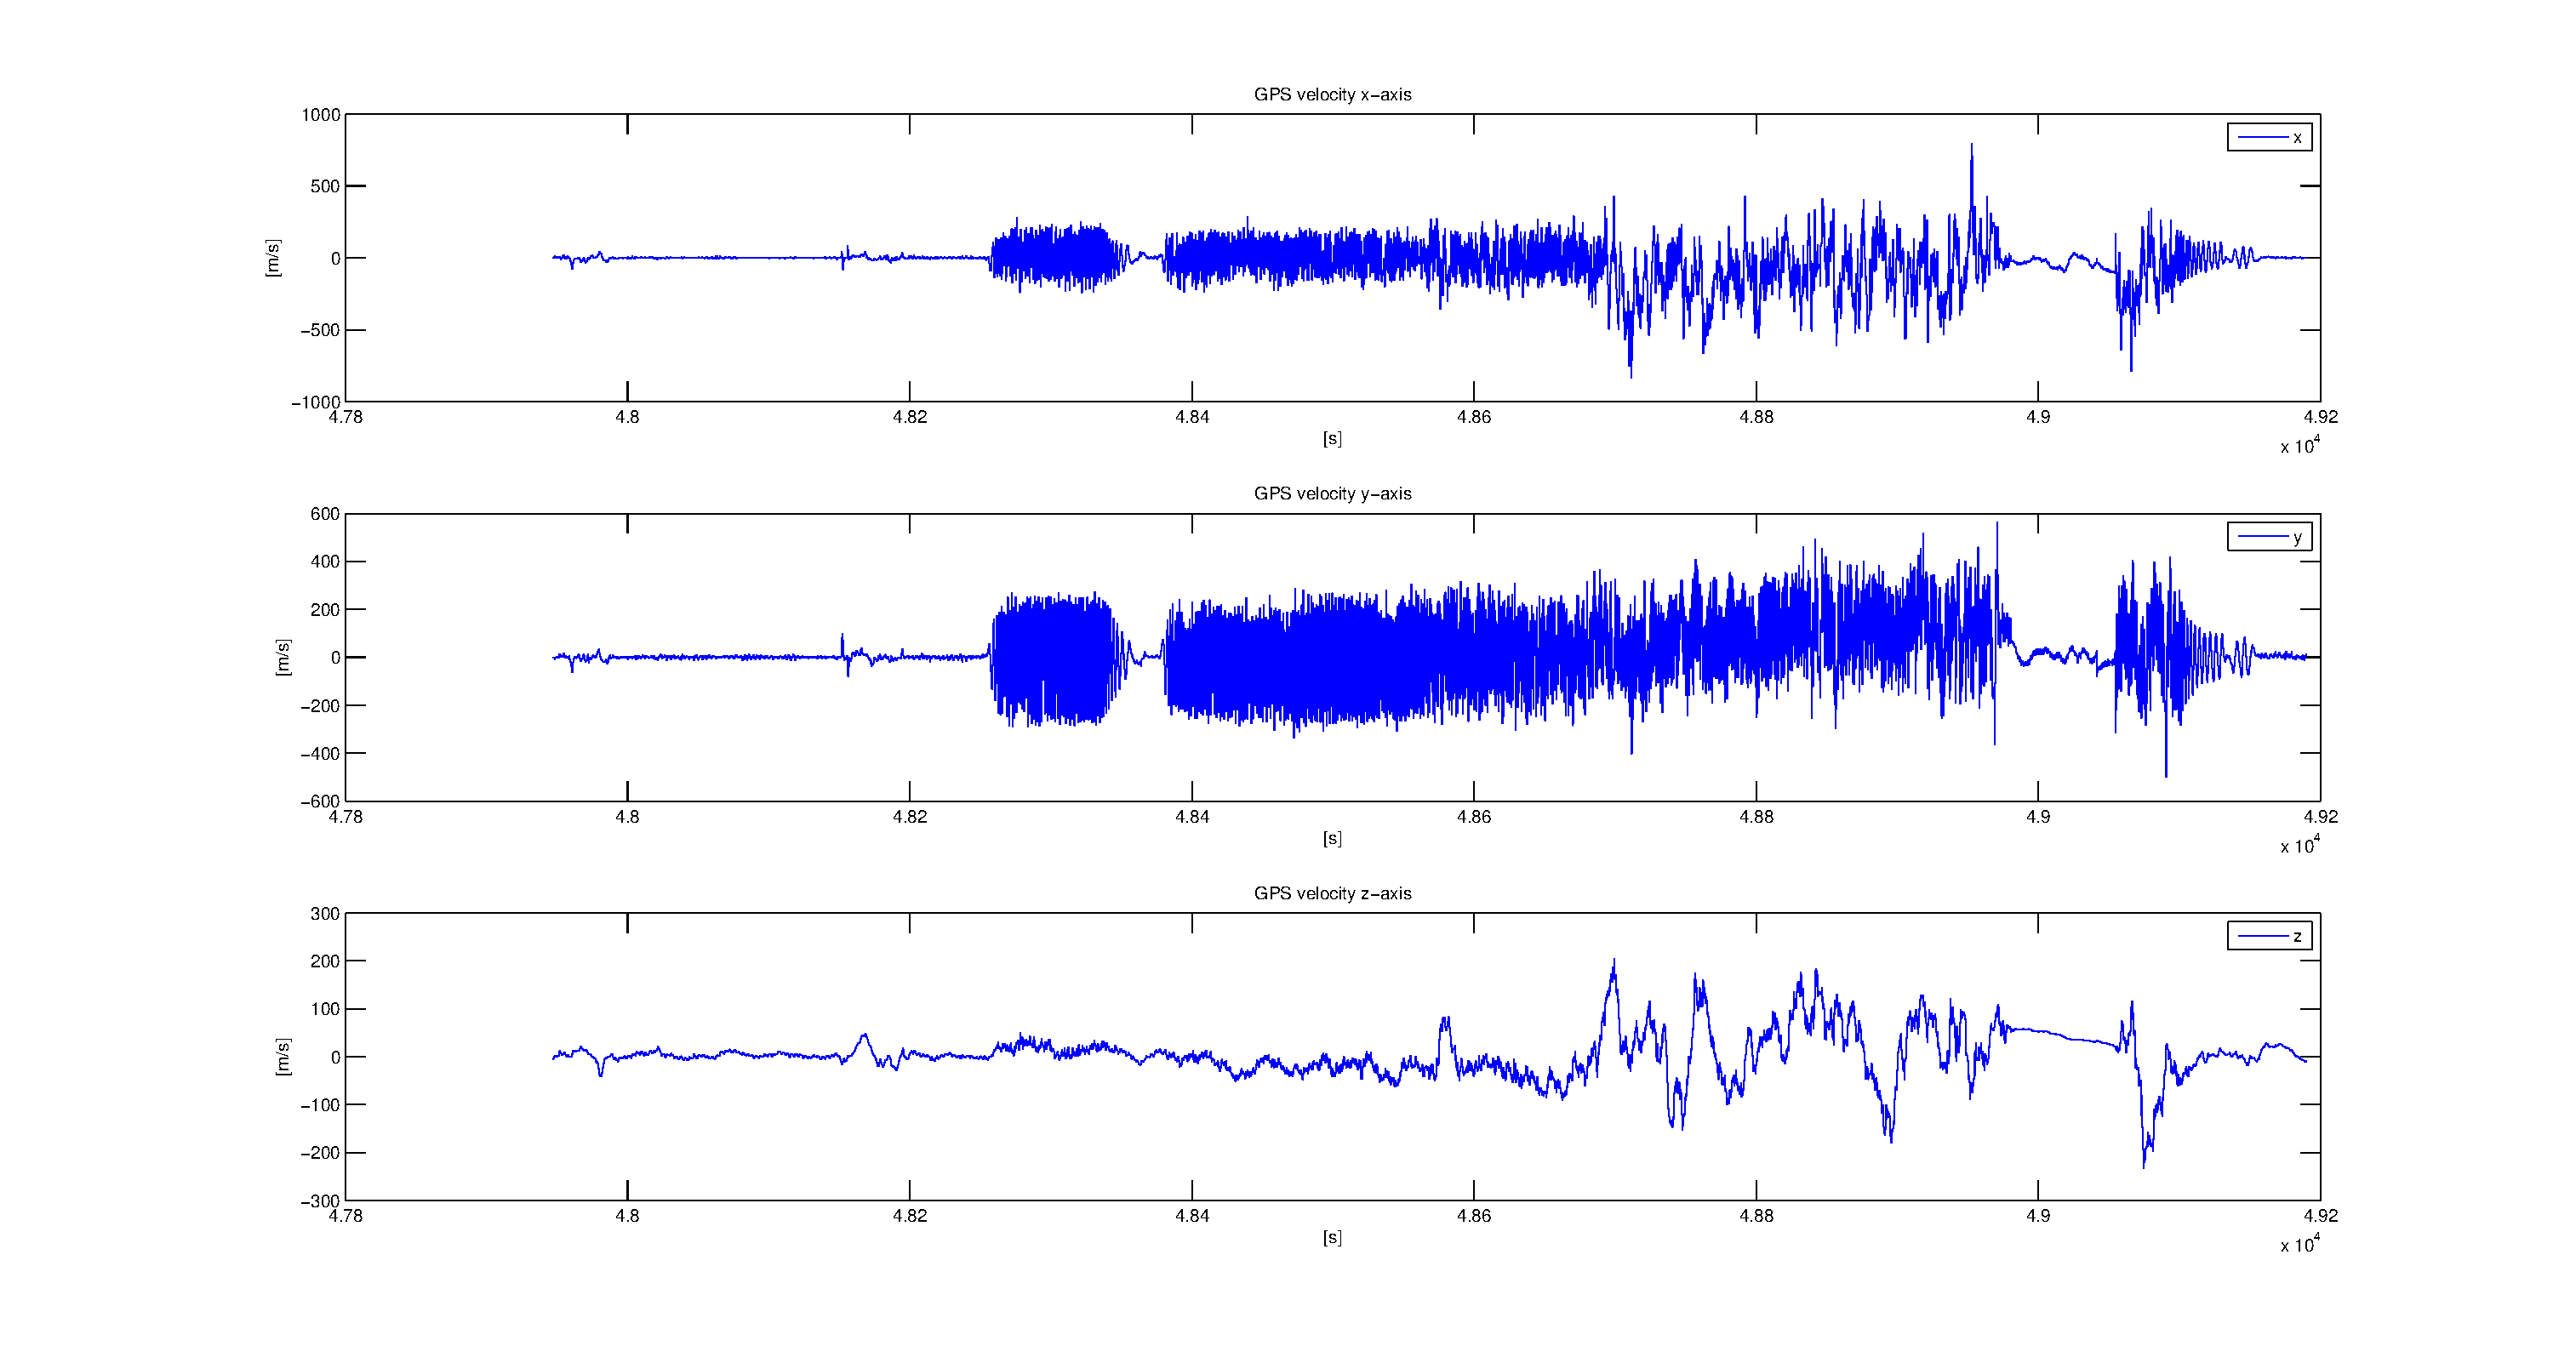
\includegraphics[width=1.2\textwidth]{pictures/ct_vel.eps}
\caption{GPS velocity}
\label{ct_vel}
\end{figure}
The periods with the correspondent average error is shown in table \ref{ct_vel_error}.
\begin{table}[h]
\centering
\begin{tabular}{|l|r|}
\hline
Period & Average error(x/y/z) \\
\hline
$4.80e4 s - 4.83e4 s$&$5.54 m / 6.05 m / 6.57 m$\\
\hline
$4.83e4 s – 4.87e4 s$&$101.86 m / 138.96 m/ 27.36 m$\\
\hline
$4.87e4s – 4.91e4 s$&$157.20 m / 123.56 m / 58.78 m$\\
\hline
\end{tabular}
\caption{The average error of the velocity in different time segments}
\label{ct_vel_error}
\end{table}
In figure \ref{ct_acc} and figure \ref{ct_gyro} the accelerometer and gyroscope measurements are shown. 
\begin{figure}[h]
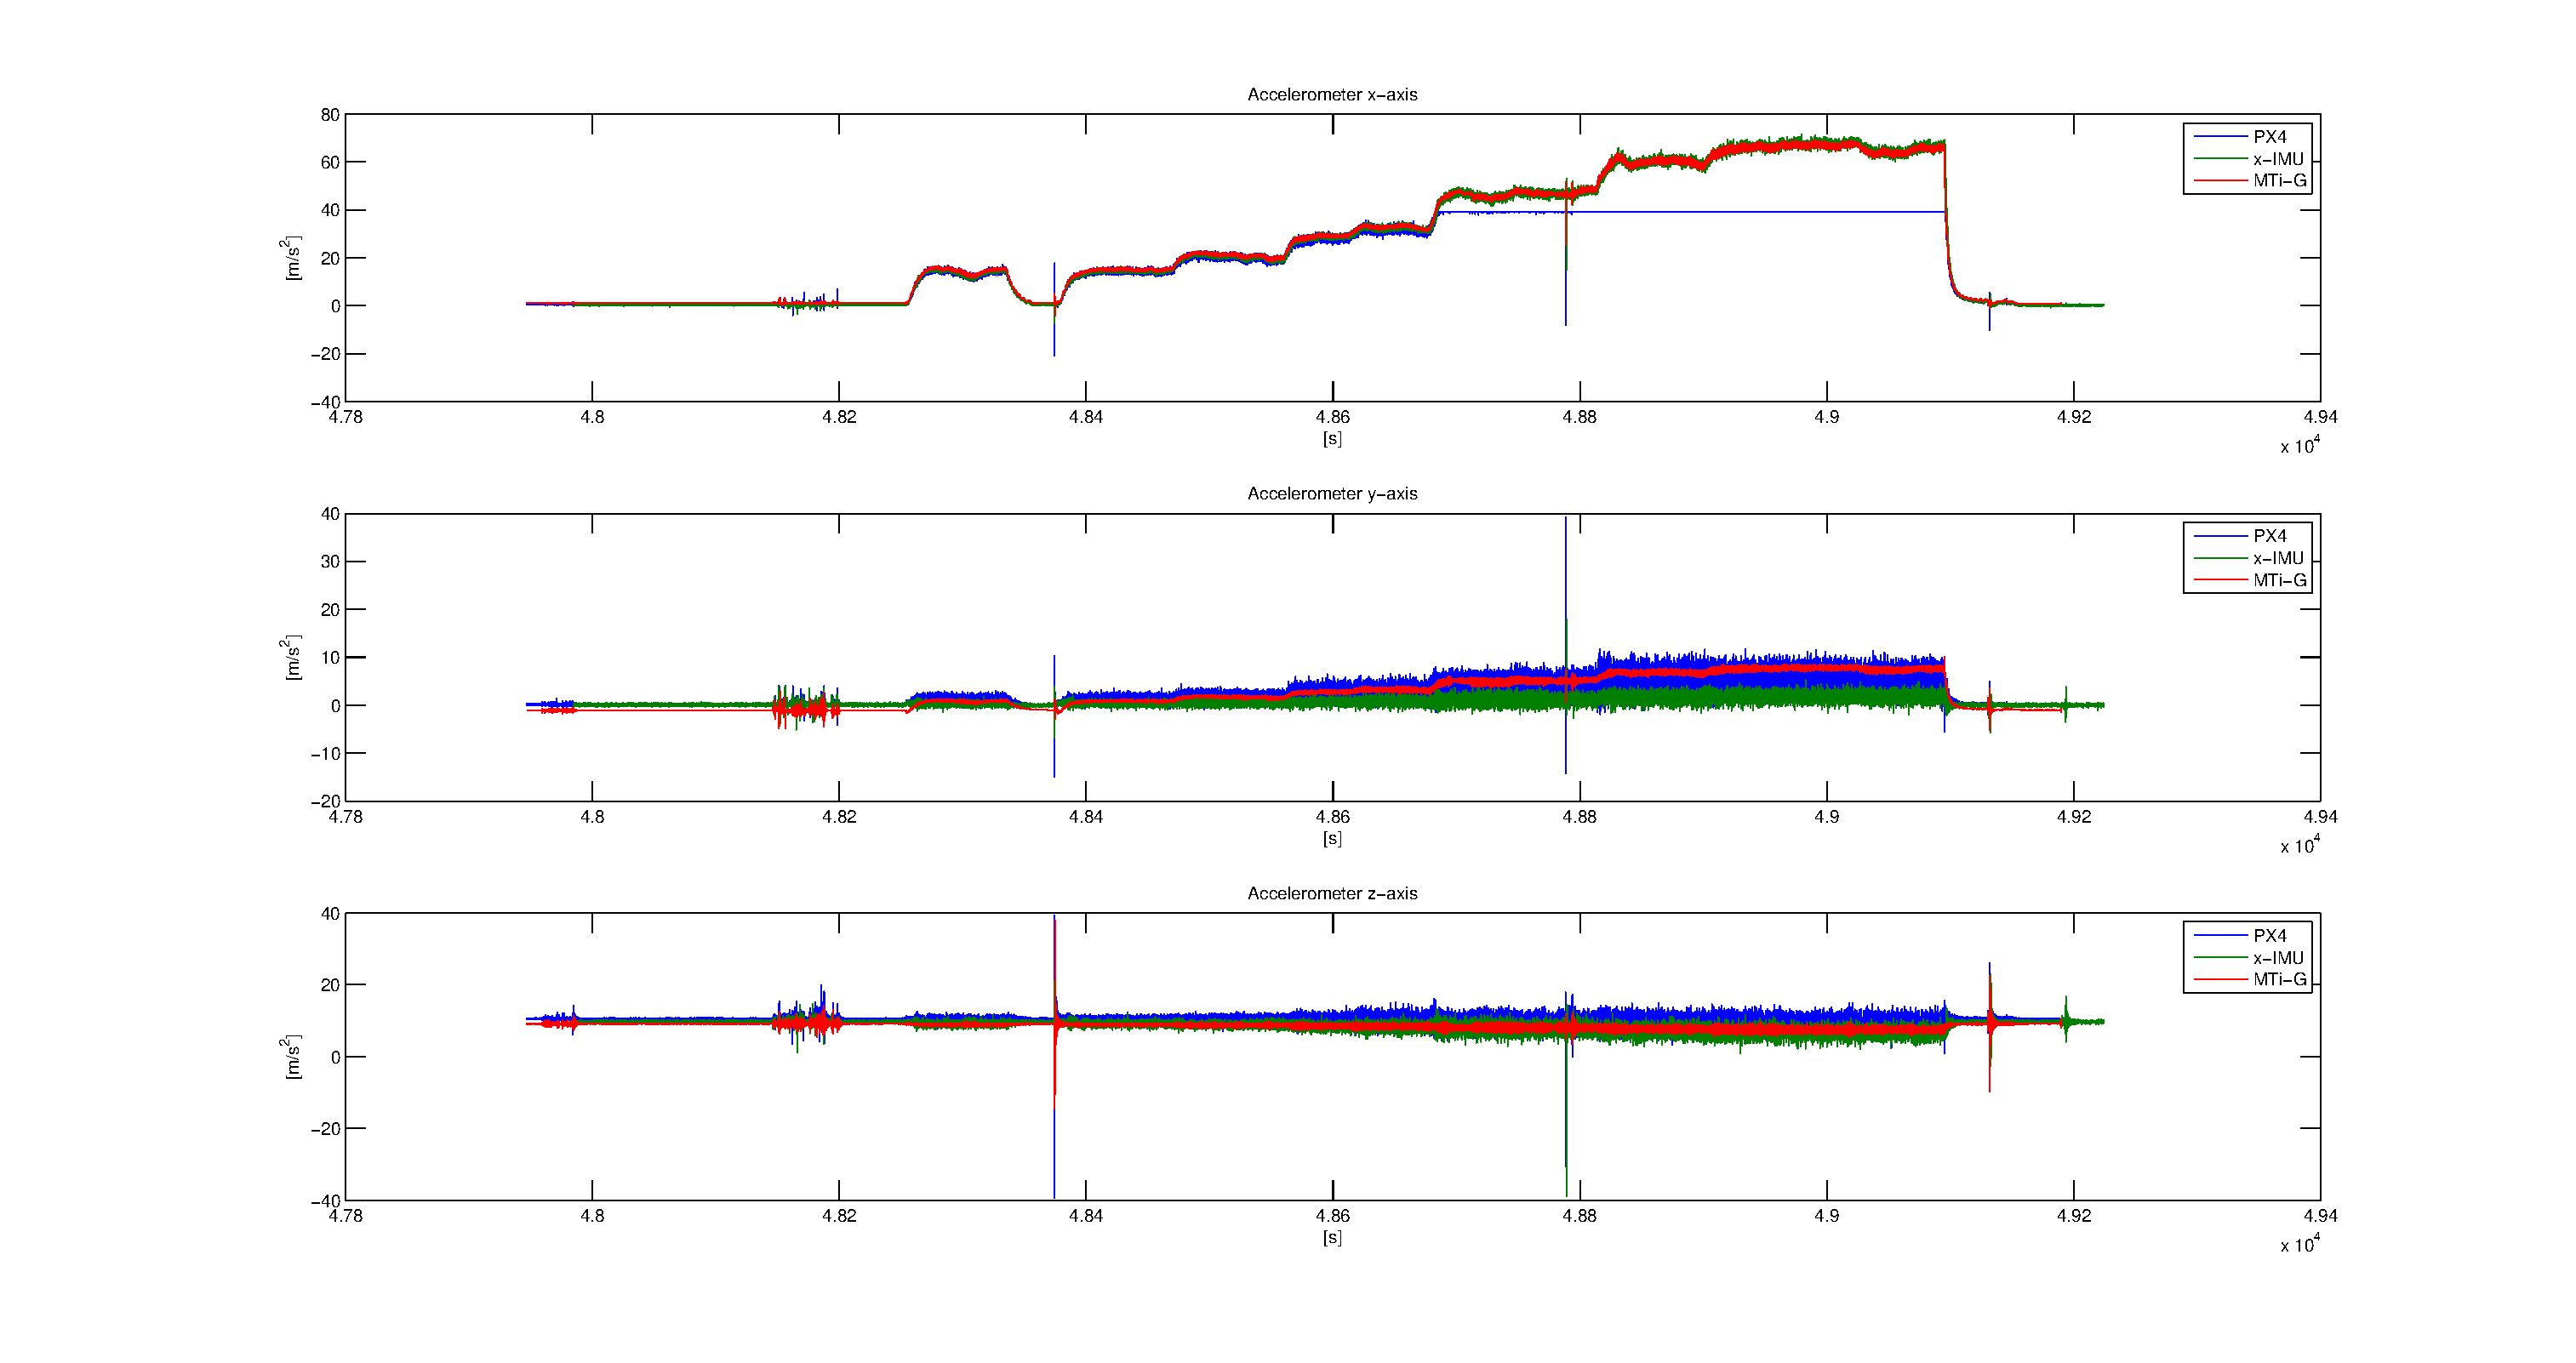
\includegraphics[width=1.2\textwidth]{pictures/ct_acc.eps}
\caption{Accelerometer}
\label{ct_acc}
\end{figure}
\begin{figure}[h]
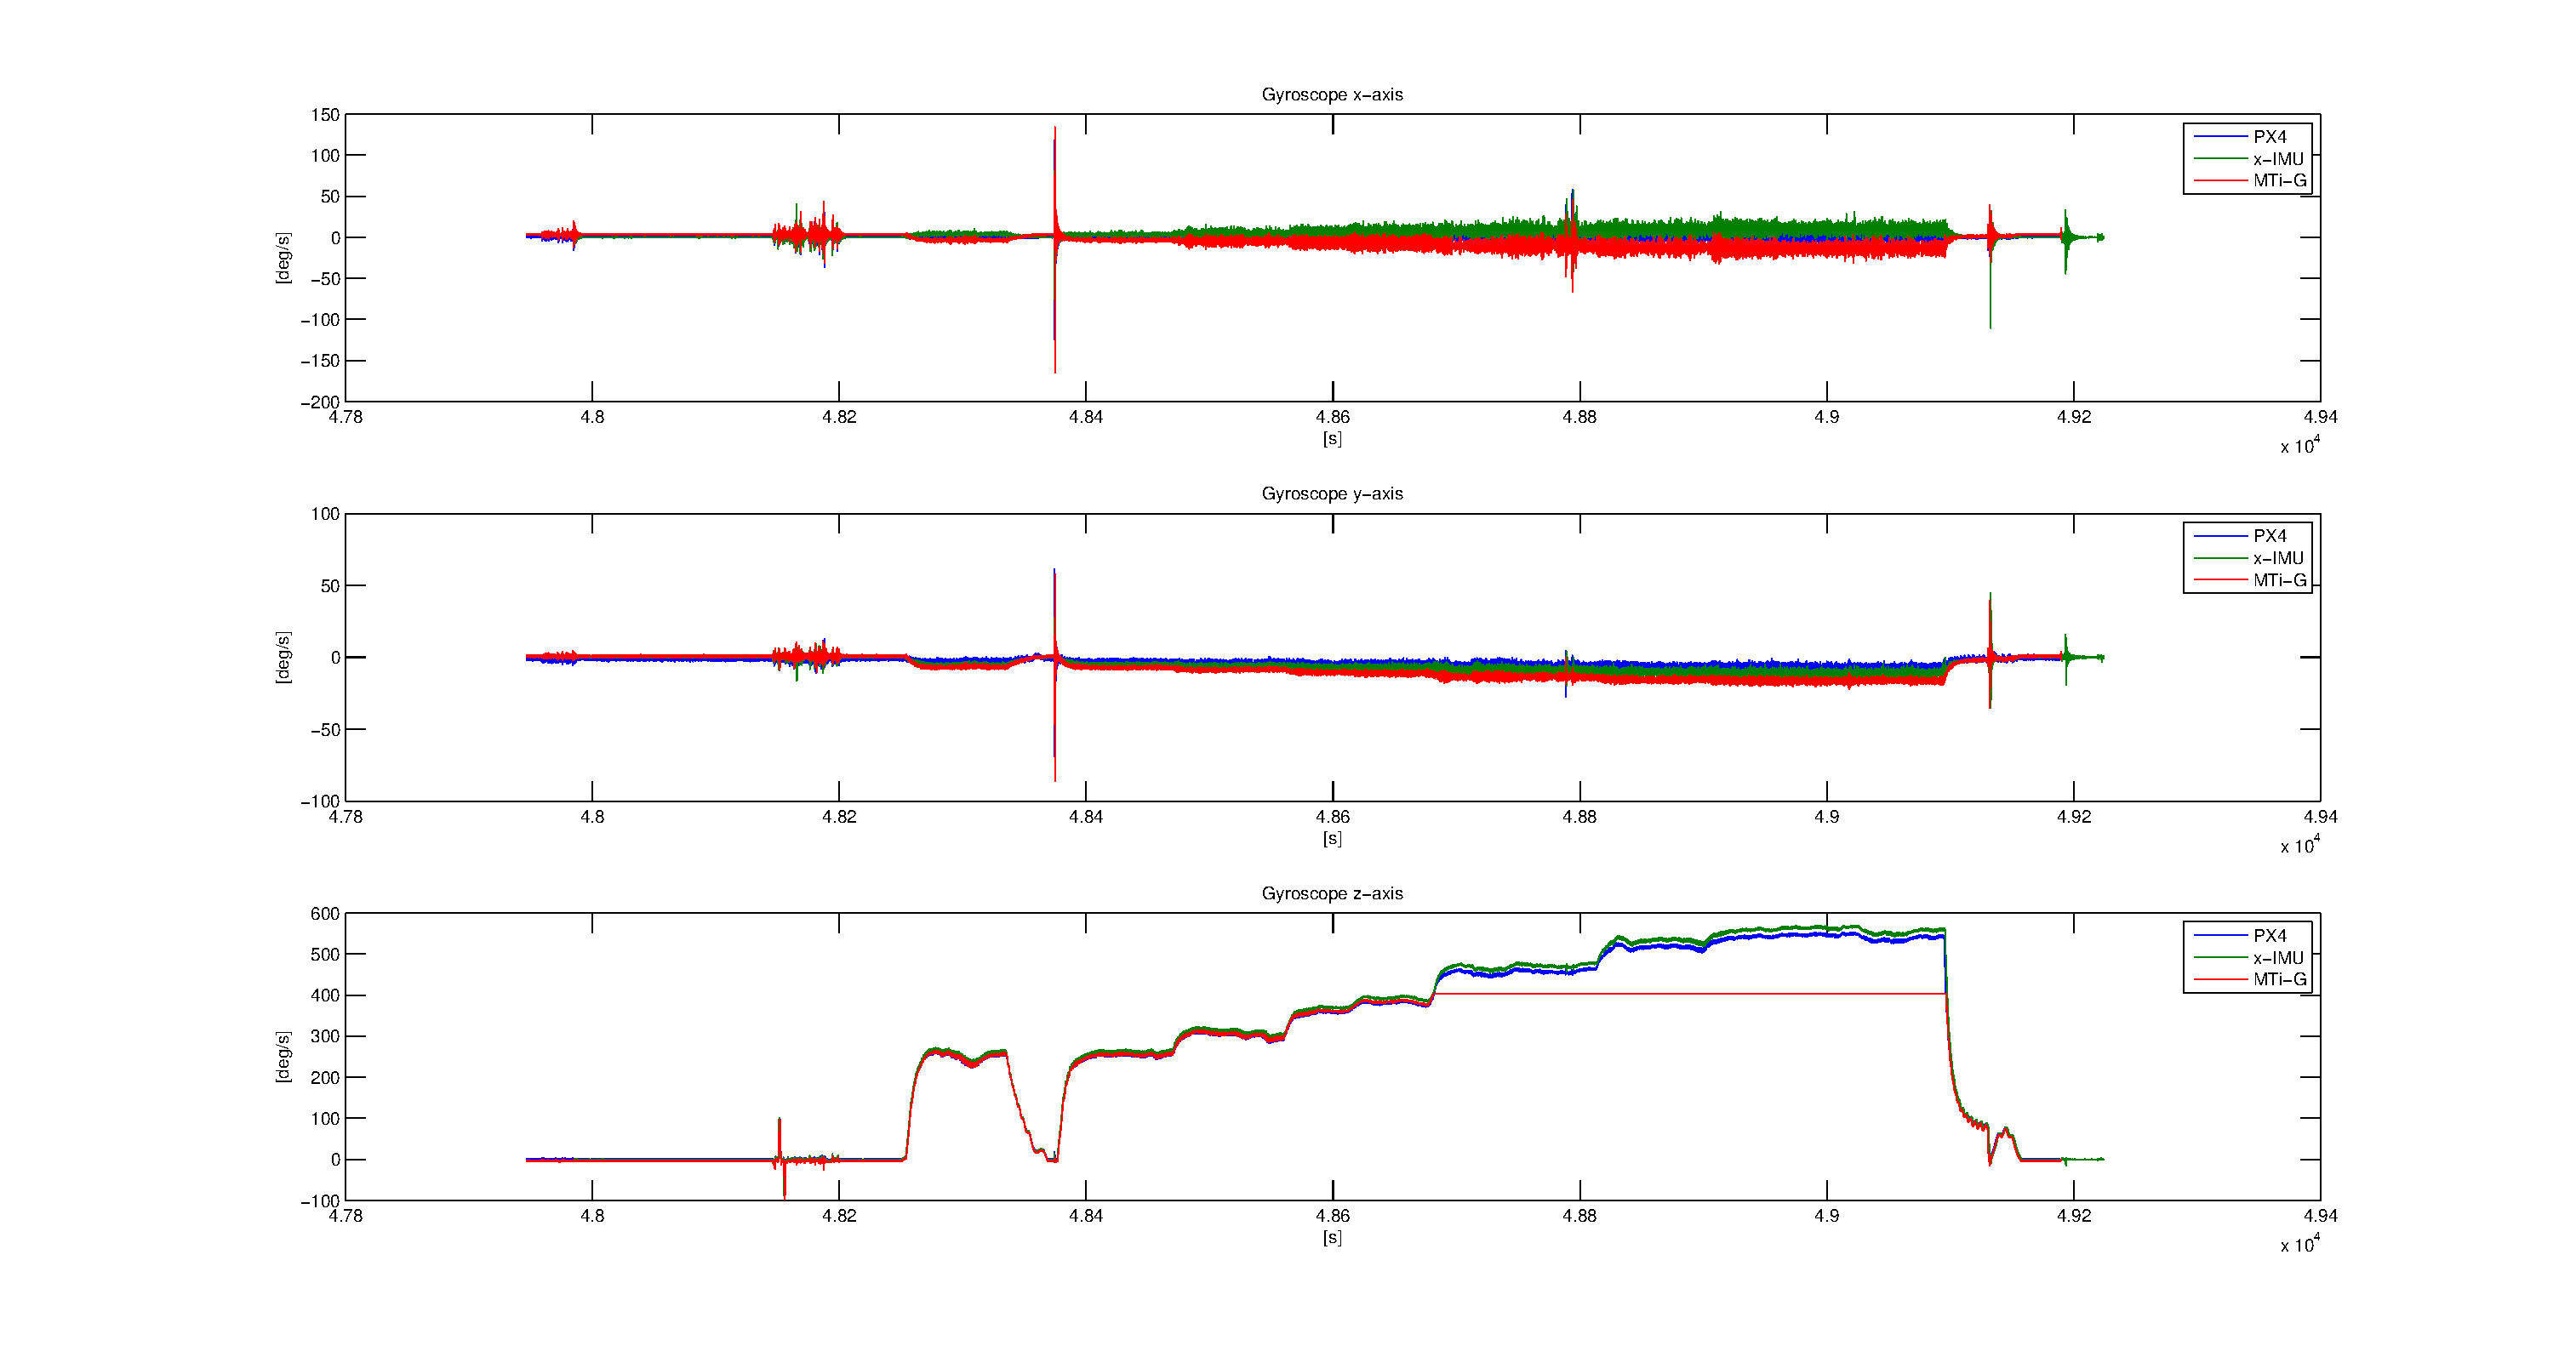
\includegraphics[width=1.2\textwidth]{pictures/ct_gyro.eps}
\caption{Gyrometer}
\label{ct_gyro}
\end{figure}
As expected, we do have the highest acceleration in x direction and the fastest rotational rate in z direction. In the accelerometer x axis and the gyroscope z axis measurements can be seen the 5 steps of different rotational speed. The very first step is a test rotation followed by the hit on the sensors which react with a peak. Since the sensitivity of the PX4 accelerometer is set to $+/- 4 g$, the output of accelerometer in x direction is limited to $39.24 m/s^2$. The acceleration in y direction is showing small steps which can be accounted for by the placement of the sensors slightly off the center of the box. The gyroscope from the MTi-G shows a limitation in measuring the rate of turn. It is unable to resolve more than $ 403 deg/s$. The x-axis and y-axis should be zero for the gyroscope since the rotation is only two dimensional. Obviously, the noise again increases with higher rates of rotation. This can be clearly seen in the acceleration in z direction which should be constant at $-9.81 m/s²$, the gravitation. It looks like the noise level of the PX4 is the highest before the x-IMU and the MTI-G which has the lowest. This can be traced back on the high sensitivity set up of the PX4 accelerometer.


In figure \ref{acc_mag} the magnetometer output is plotted.
\begin{figure}[h]
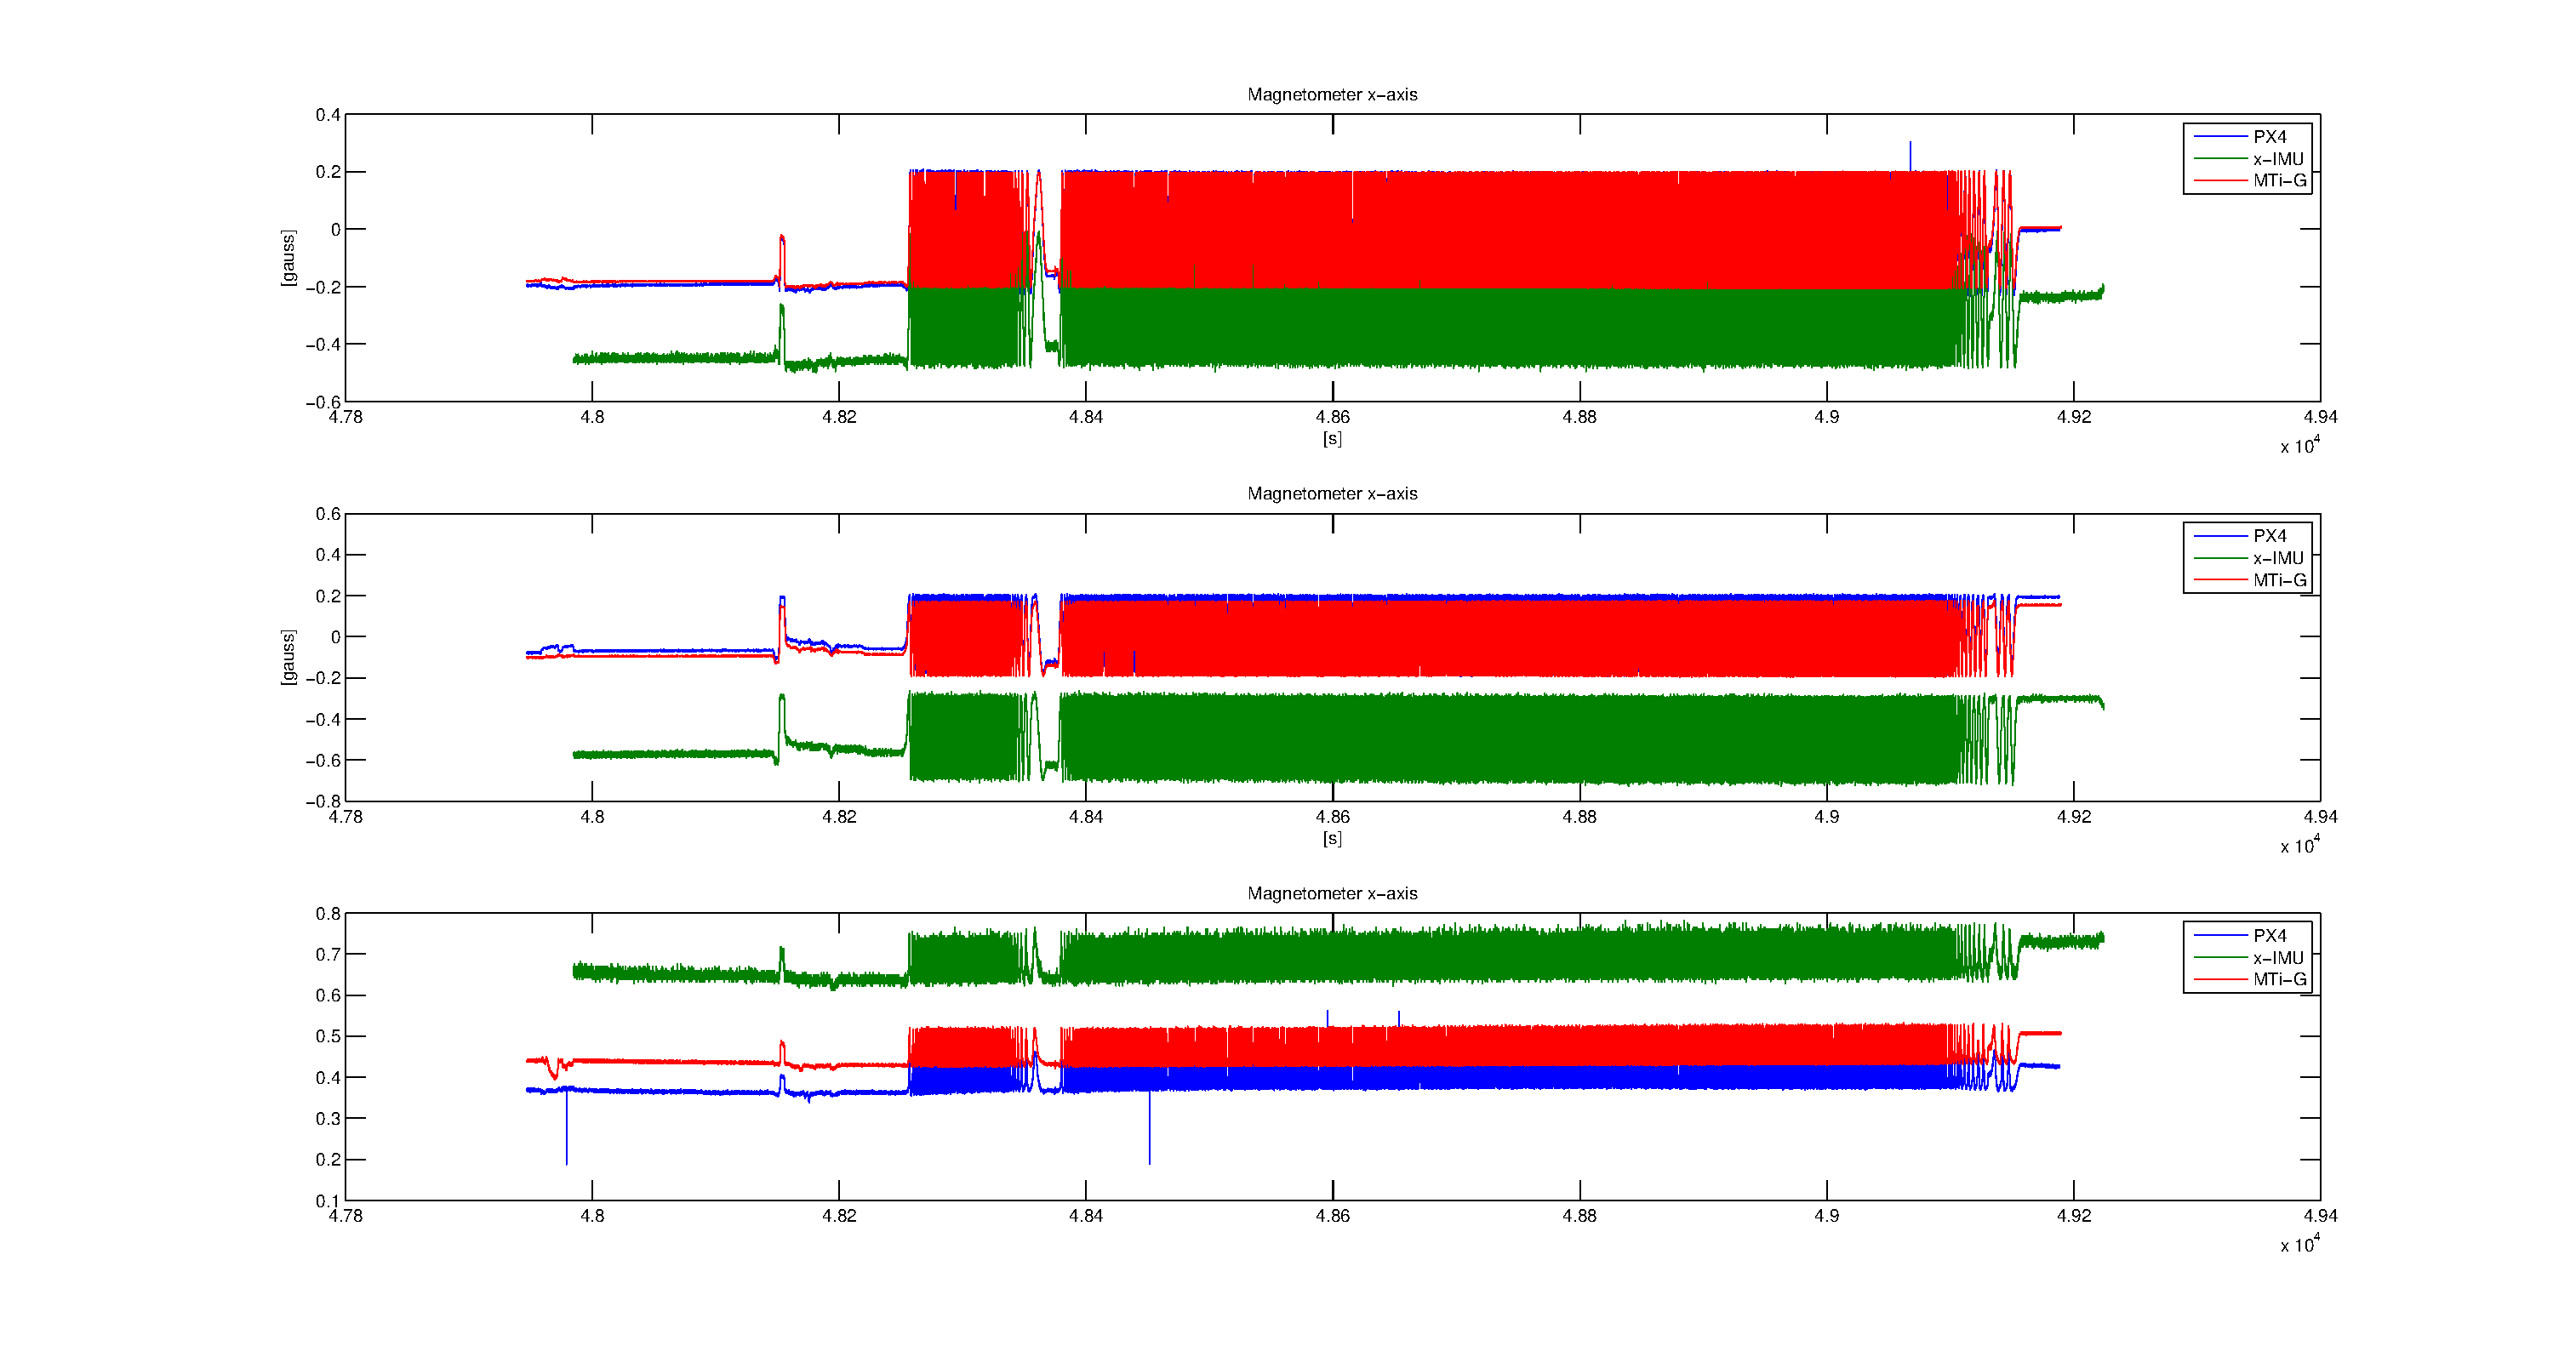
\includegraphics[width=1.2\textwidth]{pictures/ct_mag.eps}
\caption{Magnetometer}
\label{ct_mag}
\end{figure}
There is a mis alignment between the x-IMU,MTi-G and the PX4 which cannot be explained by the authors. The range of the maximum value and the minimum value of the PX4, MTi-G and the x-IMU is in x and y direction $0.4 gauss$. This is the expected range in the region of Zurich. In this sense, if the the output is added with an offset in order to get the range to $+/- 0.2 gauss$, the measurements should be correct. The PX4 has a mean value of $0.3893$ gauss while the ground truth is $0.4268 gauss$.  The noise of the magnetometer is in the x-IMU higher than in the other two IMUs.

In figure \ref{ct_sine} a closer look on the x axis of the magnetometer and accelerometer and on the y axis of the gyroscope is presented. The form of the curve has sine behavior, what we would expect again.
\begin{figure}[h]
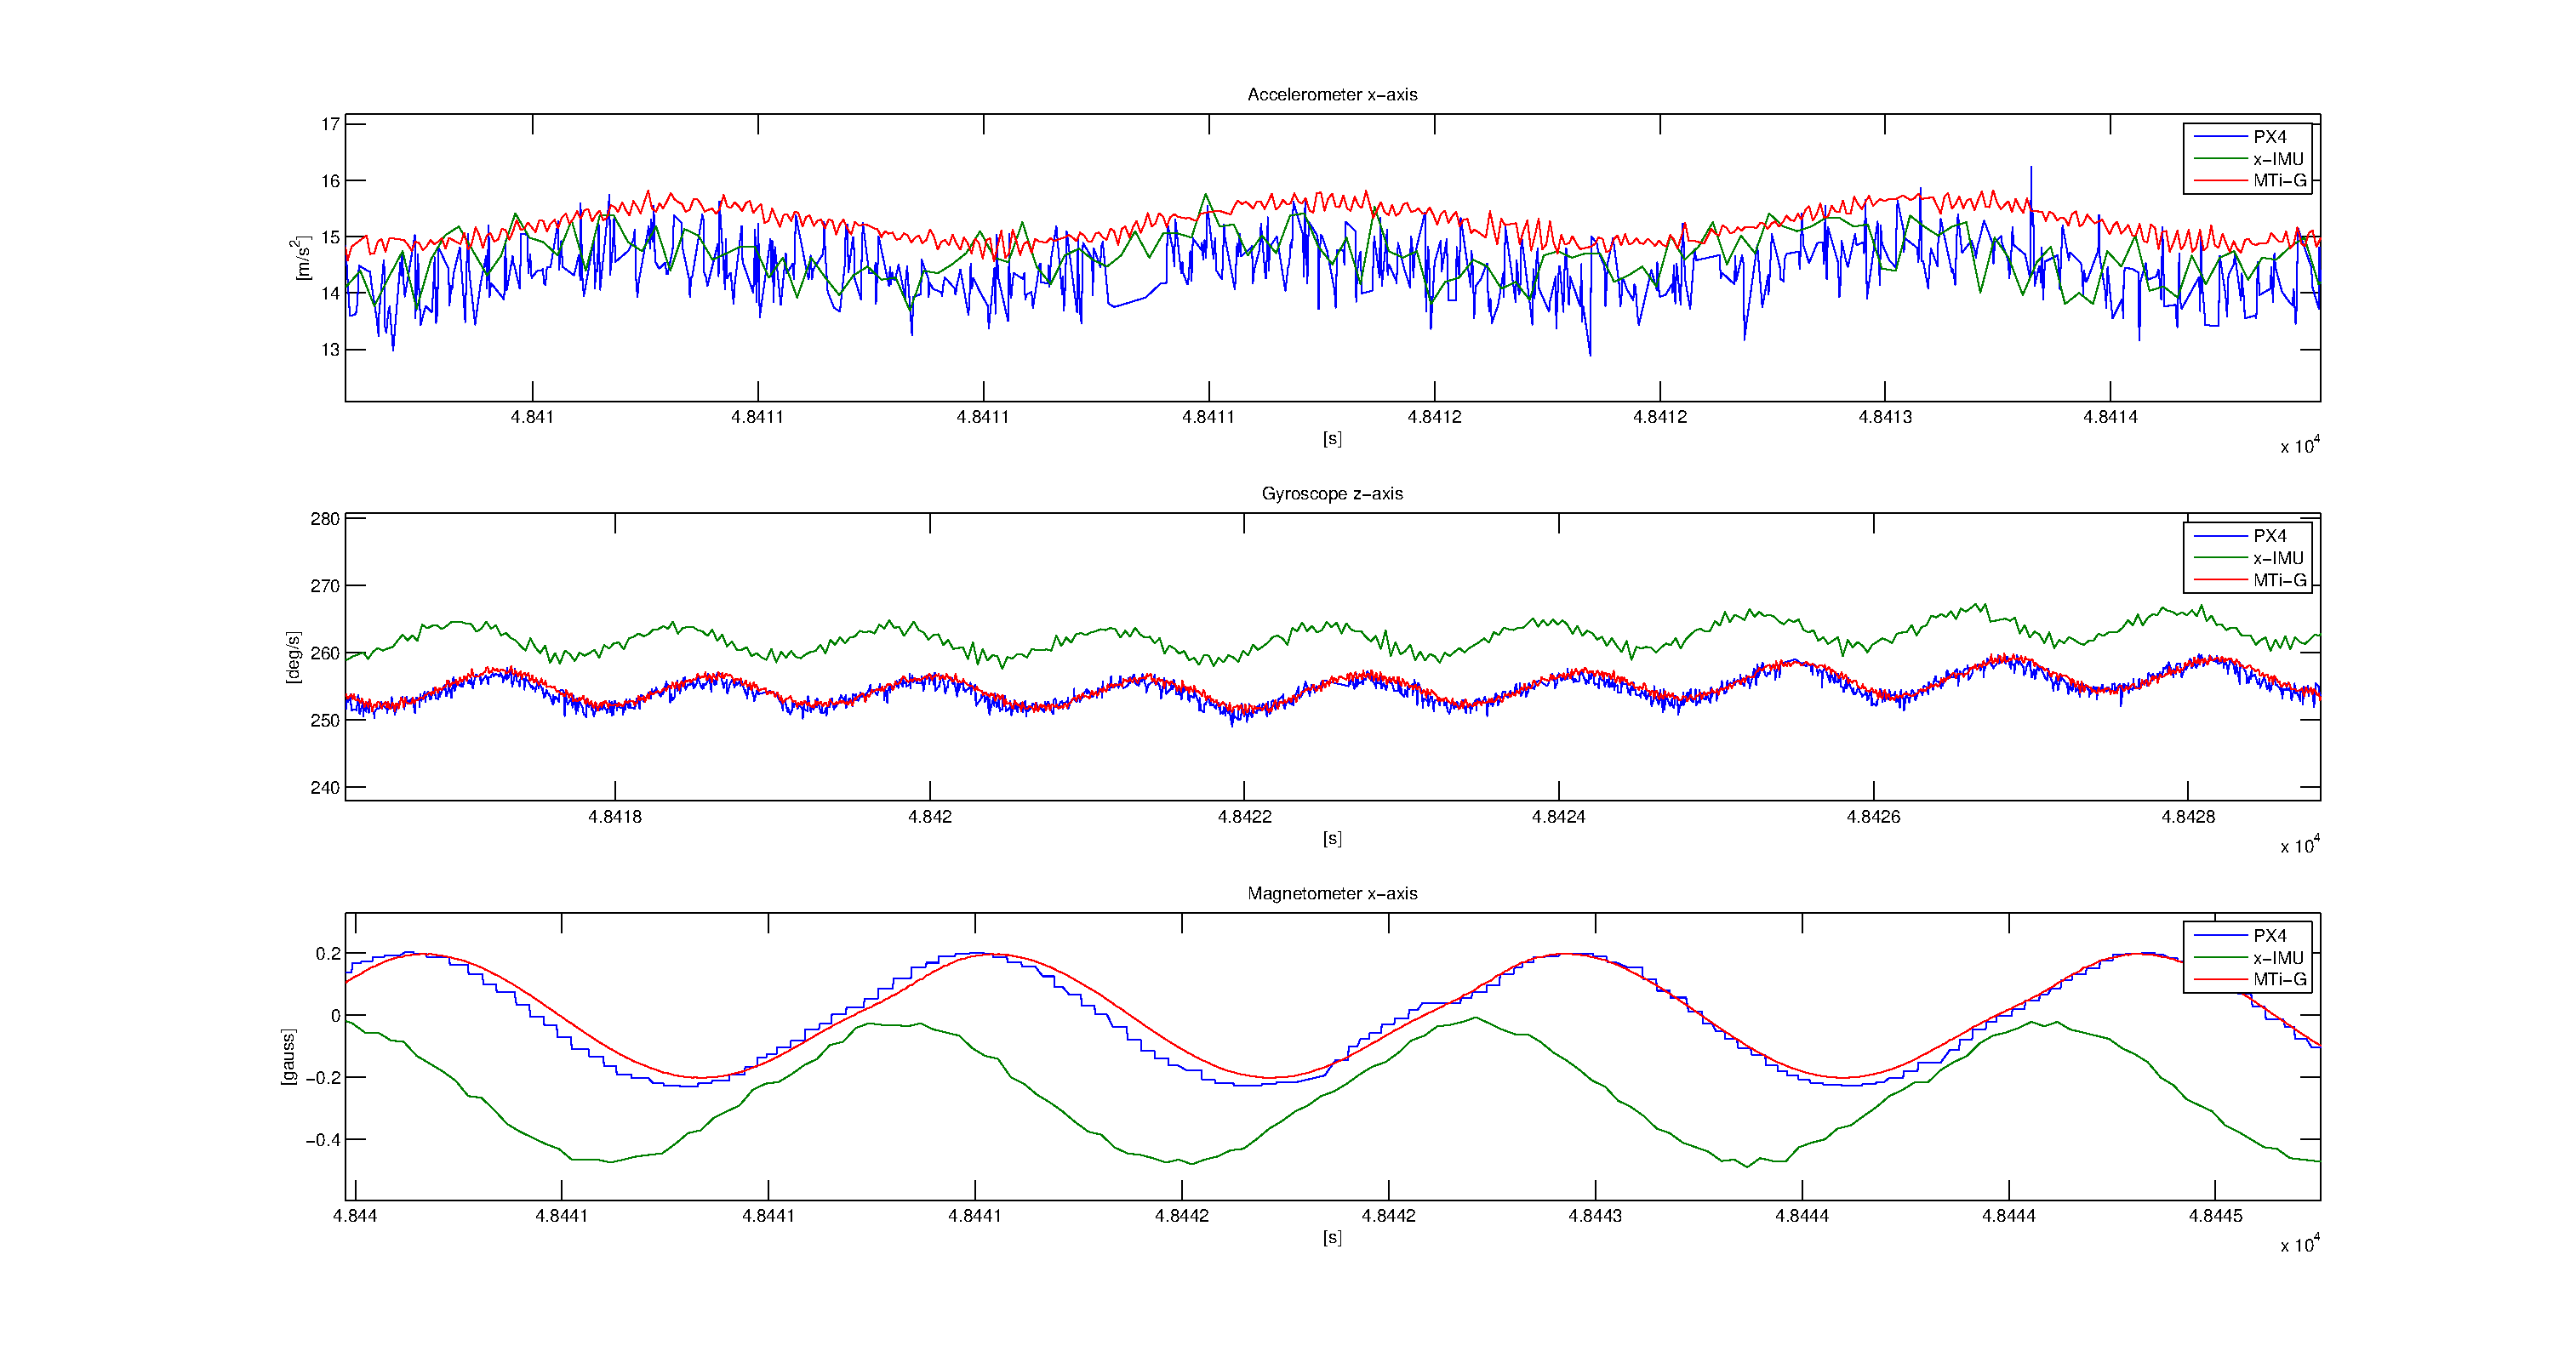
\includegraphics[width=1.2\textwidth]{pictures/ct_sine.eps}
\caption{A closer look in time on the three IMU sensors.}
\label{ct_sine}
\end{figure}

\subsection{Conclusion}
All IMUs work in the same range of noise level. With an increasing rotational velocity and therefore a higher centripetal acceleration, the average error is increasing in all sensors, except in the magnetometer. There could not be found a dependency between noise in the measurement of the magnetic field and the acceleration. 
In a future experiment it would be interesting to also record the rotational rate of the centrifuge in order to have a more accurate ground truth that could be used to determine the accuracy of the IMU measurements. This could lead to a more founded compairison of the the different sensors' accuracy. Finally the sensitivity of the accelerometer of the PX4 unit should be set in a way to be able to observe the whole range of the applied centripetal acceleration and the MTi-G would need to be set to record the data in the calibrated output mode.

